\documentclass[conference]{IEEEtran}

\ifCLASSINFOpdf
 
\else
  
\fi

\hyphenation{op-tical net-works semi-conduc-tor}
\usepackage{amsmath}
\usepackage{graphicx}
\usepackage{float}
\usepackage{subfig}
\usepackage{xcolor}
\usepackage[colorlinks = true,
            linkcolor = blue,
            urlcolor  = blue,
            citecolor = blue,
            anchorcolor = blue]{hyperref}
\usepackage{mathtools}

\begin{document}

\title{CMSC733 - Project 2\\Face Swap}

\author{\IEEEauthorblockN{Saurabh Palande}
\IEEEauthorblockA{Masters in Robotics\\
University of Maryland, College Park\\
UID: 118133959\\
Email: spalande@umd.edu\\}
\and

\IEEEauthorblockN{Nishad Kulkarni}
\IEEEauthorblockA{Masters in Robotics\\
University of Maryland, College Park\\
UID: 117555431 \\
Email: nkulkar2@umd.edu}}
\maketitle

\begin{abstract}
The aim of this project is to implement an end-to-end pipeline to swap faces in a video just like Snapchat’s face swap filter or any face swap website. This is a fairly complicated procedure and variants of the approach implemented in this project have been used in many movies. The first approach is the traditional approach which consists of 2 methods: 1. Using Delaunay Triangulation and Barycentric coordinates 2.Using Thin Plate Spline. The second approach is the Deep learning approach to obtain face fiducials/full 3D mesh and then perform face replacement.
\end{abstract}

\IEEEpeerreviewmaketitle

\section{Phase I - Traditional Approach}
The traditional approach consist of 4 important steps which are detecting face fiducials, Warping to other face, replacing the face and then performing blending. The complete pipeline is mentioned in Figure 1.
\begin{figure}[H]
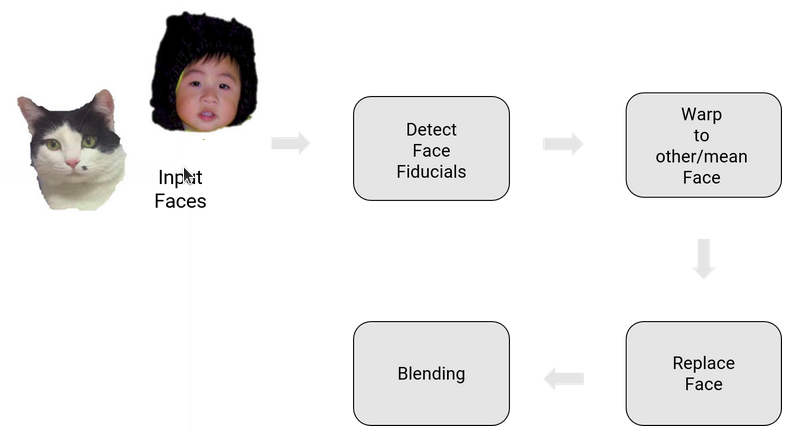
\includegraphics[scale=0.3]{pipeline.png}
\centering
\caption{Face swap pipeline}
\end{figure}
The two traditional methods of face warping used in this project are:
\begin{enumerate}
\item Face warping using Delaunay Triangulation
\item Face warping using Thin Plate Spline
\end{enumerate}

\subsection{Detecting Facial Landmarks}
The first step in the traditional approach is to find facial landmarks (important points on the face) so that there is one-to-one correspondence between the facial landmakrs. One of the major reasons to use facial landmarks instead of using all the points on the face is to reduce computational complexity though better results can be obtained using all the points (dense flow) or using a meshgrid. For detecting facial landmarks dlib library built into OpenCV and Python is used. The detected facial landmarks of the target and source face is shown in the Figure 2 and Figure 3 respectively.
\begin{figure}[H]
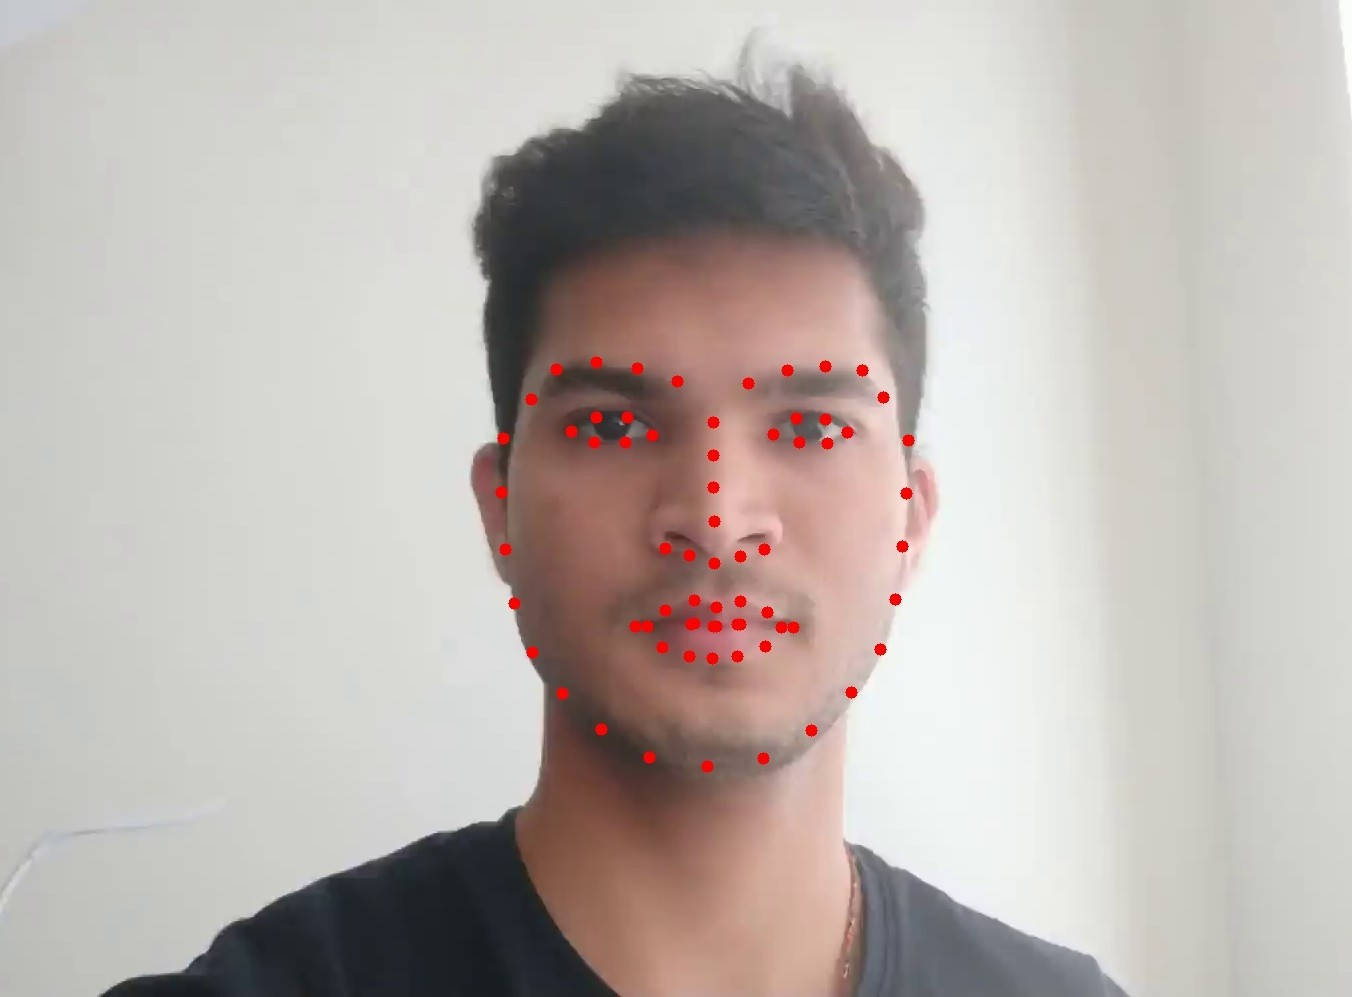
\includegraphics[scale=0.2]{f_t.jpg}
\centering
\caption{Facial landmarks of Target face}
\end{figure}
\begin{figure}[H]
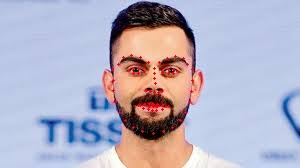
\includegraphics[scale=0.9]{f_s.jpg}
\centering
\caption{Facial landmarks of Source face}
\end{figure}
\subsection{Face Warping}
Now that the facial landmarks are detected, the next step is to warp the target and source faces using these landmarks. The two methods used in this project are:
\subsubsection{Using Delaunay Triangulation}
To swap the faces we need to warp the faces in 3D, however we don’t have 3D information. So we make some assumption about the 2D image to approximate 3D information of the face by triangulation using the facial landmarks as corners and assuming that in each triangle the content is planar and hence the warping between the triangles in two images is affine. Delaunay Triangulation is used as it tries to maximize the smallest angle in each triangle. Since we use dlib to find the facial landmarks, there is correspondence between the facial landmarks and hence correspondence between the triangles.
The generated delaunay triangles of the source and the target image is shown in Figure and figure respectively.
\begin{figure}[H]
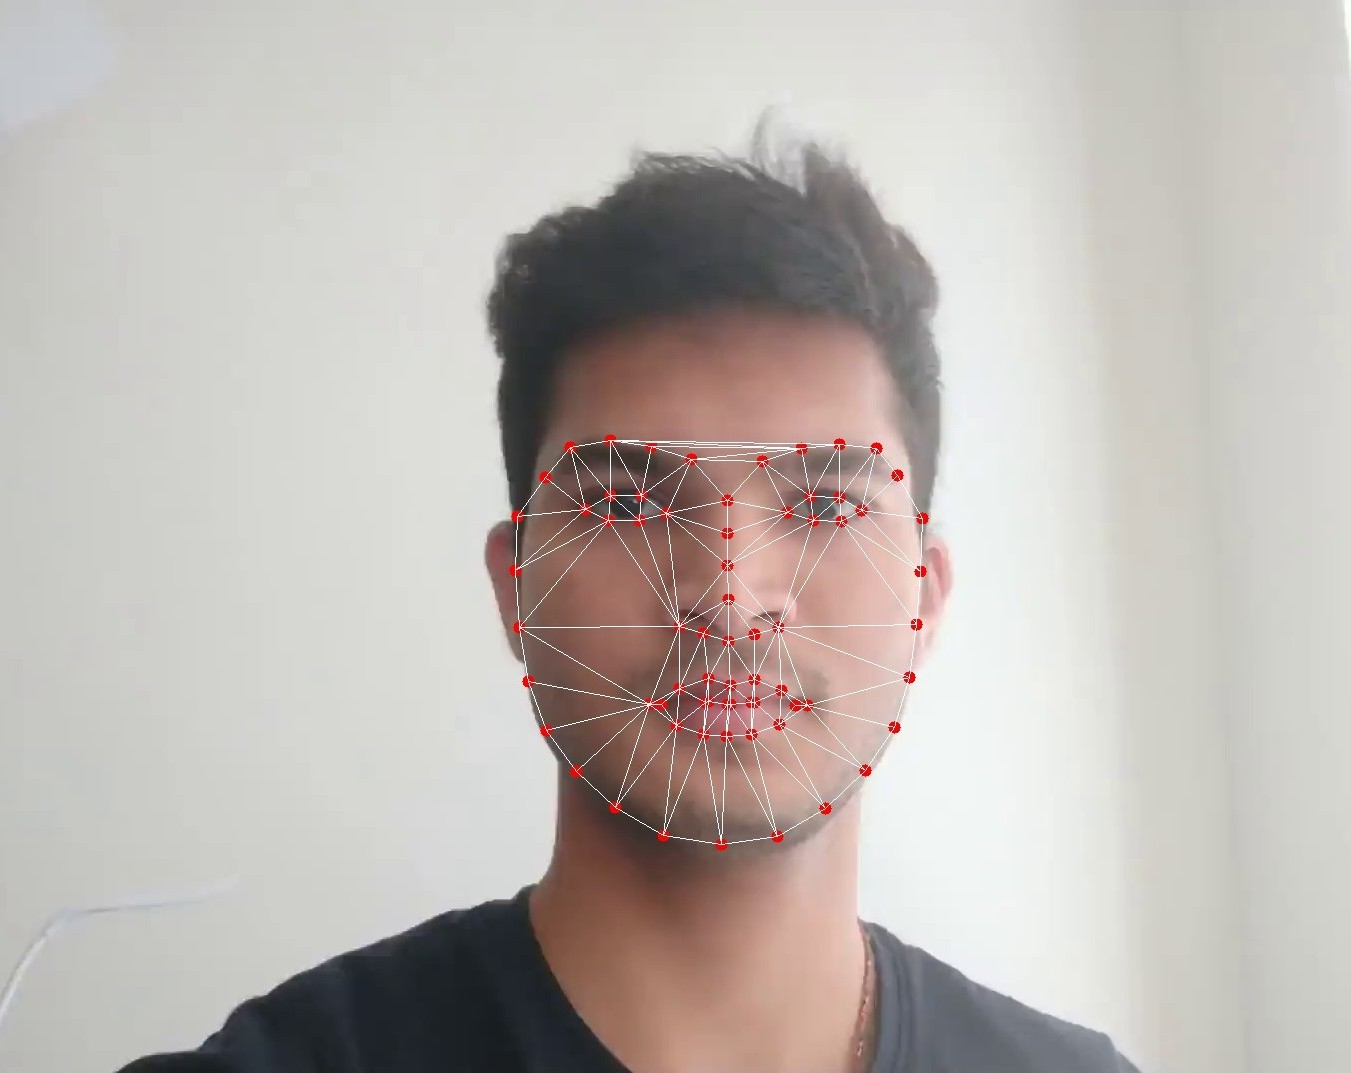
\includegraphics[scale=0.18]{dt.jpg}
\centering
\caption{Delaunay triangle of Target face}
\end{figure}
\begin{figure}[H]
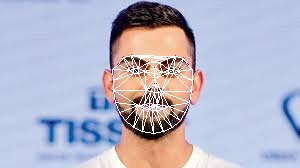
\includegraphics[scale=0.85]{ds.jpg}
\centering
\caption{Delaunay triangle of Source face}
\end{figure}
To warp one face to another the following steps are followed:
\begin{enumerate}
\item For each triangle in the target/destination face B, compute the Barycentric coordinate.
\begin{equation}
\begin{bmatrix}
B_{ax} & B_{bx} & B_{cx} \\
B_{ay} & B_{by} & B_{cy} \\
1 &1 &1
\end{bmatrix}
\begin{bmatrix}
\alpha \\
\beta \\
\gamma
\end{bmatrix}
= 
\begin{bmatrix}
x\\
y\\
1
\end{bmatrix}
\end{equation}
Given a point (x,y,1), the barycentric coordinates can be found as
\begin{equation}
\begin{bmatrix}
\alpha\\
\beta\\
\gamma
\end{bmatrix}
=
{B_{\Delta}}^{-1}
\begin{bmatrix}
x\\
y\\1
\end{bmatrix}
\end{equation} 
The point (x,y,1) lies inside the triangle if $\alpha$, $\beta$, $\gamma$ lie in [0,1] and $\alpha + \beta + \gamma$ lies in (0,1].
\item Now that we have the barycentric coordinate, we can find the corresponding pixel position on the source image.
\begin{equation}
\begin{bmatrix}
x_{A}\\
y_{A}\\
z_{A}
\end{bmatrix}
= 
A_{\Delta}
\begin{bmatrix}
\alpha\\
\beta\\
\end{bmatrix}
\end{equation}
where
\begin{equation}
A_{\Delta} = 
\begin{bmatrix}
A_{ax} & A_{bx} & A_{cx} \\
A_{ay} & A_{by} & A_{cy} \\
1 &1 &1
\end{bmatrix}
\end{equation}
\item After obtaining ${\begin{bmatrix}
x_A & y_A & z_A
\end{bmatrix}^T}$, we need to convert them to homogeneous coordinates as follows
\begin{equation}
x_A = \frac{x_A}{z_A}
\end{equation}  
\begin{equation}
y_A = \frac{y_A}{z_A}
\end{equation} 
\item Copy the value of pixel at $(x_A, y_A)$ to the target location. For this scipy.interpolate.interp2d is used.
\end{enumerate} 
\subsubsection{Using Thin Plate Spline}
Face warping using triangulation assumes that we are doing affine transformation on each triangle. This might not be the best way to do warping since the human face has a very complex and smooth shape. A better way to do the transformation is by using Thin Plate Splines (TPS) which can model arbitrarily complex shapes. We compute a TPS that maps from the feature points in B to the corresponding feature points in A . We define two splines, one for the x coordinate and one for the y having the following form:
\begin{equation}
f(x,y) = a_1 + (a_x)x + (a_y)y + \sum_{\mathclap{i=1}}^{p} w_{i}U(||(x_i, y_i) - (x,y)||_1)
\end{equation}
where $U(r) = r^{2}log(r^2)$
We find the parameters of a Thin Plate Spline which will map from B to A. Warping using a TPS is performed in two steps which are as follows:
\begin{enumerate}
\item In the first step, we will estimate the parameters of the TPS. The solution of the TPS model requires solving the following equation:
\begin{equation}
\begin{bmatrix}
K & P \\
P_T & 0
\end{bmatrix}
\begin{bmatrix}
w_1\\
w_2\\
:\\
:\\
w_p\\
a_x\\
a_y\\
a_1
\end{bmatrix}
=
\begin{bmatrix}
v_1\\
v_2\\
:\\
:\\
v_p\\
0\\
0\\
0
\end{bmatrix}
\end{equation}

\begin{equation}
\begin{bmatrix}
w_1\\
w_2\\
:\\
:\\
w_p\\
a_x\\
a_y\\
a_1
\end{bmatrix}
=
(
\begin{bmatrix}
K & P \\
P_T & 0
\end{bmatrix}
+ \lambda I(p+3, p+3))^{-1}
\begin{bmatrix}
v_1\\
v_2\\
:\\
:\\
v_p\\
0\\
0\\
0
\end{bmatrix}
\end{equation}
\item In the second step, we use the estimated parameters of the TPS models (both x and y directions) and transform all pixels in image B by the TPS model. Then we read back the pixel value from image A directly. The position of the pixels in image A is generated by the TPS equation. The output images are shown in the figures below:
\begin{figure}[H]
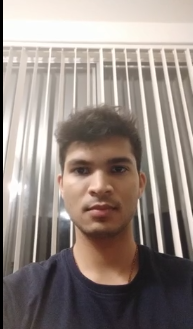
\includegraphics[scale=0.4]{1.png}
\centering
\caption{Original image}
\end{figure}
\begin{figure}[H]
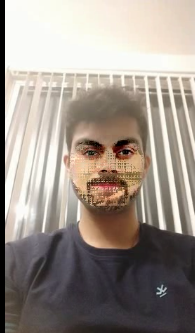
\includegraphics[scale=0.4]{dt11.png}
\centering
\caption{Swapped face by Delaunay}
\end{figure}
\begin{figure}[H]
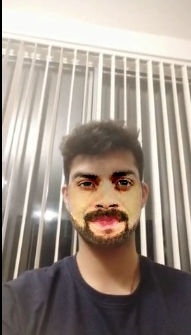
\includegraphics[scale=0.4]{tps1.png}
\centering
\caption{Swapped face by TPS}
\end{figure}
\begin{figure}[H]
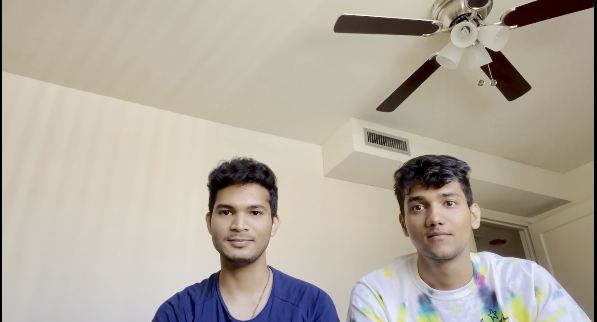
\includegraphics[scale=0.4]{tps2.png}
\centering
\caption{Original image}
\end{figure}
\begin{figure}[H]
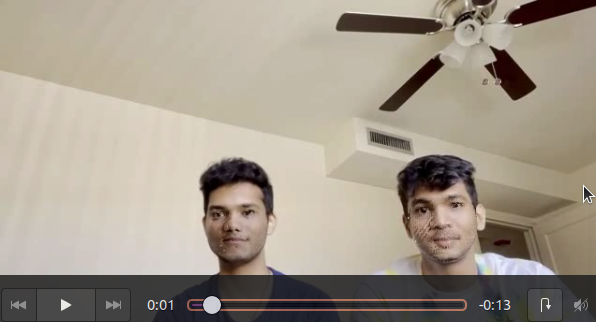
\includegraphics[scale=0.4]{dt2.png}
\centering
\caption{Swapped face by Delaunay}
\end{figure}
\begin{figure}[H]
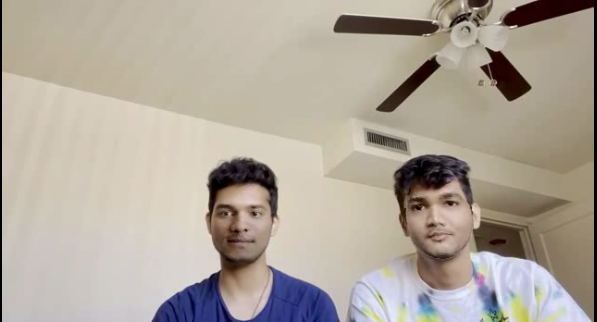
\includegraphics[scale=0.4]{tps2swap.png}
\centering
\caption{Swapped face by TPS}
\end{figure}
\end{enumerate}hat w

\section{Phase II - PRNet}

The Deep Learning approach of this project involve using the PRNet Neural Network proposed by Yao Feng, et al. in their paper [1]. The code[2] for this was provided by the authors themselves. We Modified that code to make it swap faces detected in a video with a reference image that the user provides. Also, we modified it to swap faces in a given video. Below we can see the results of various swaps that were performed. (Please note that this task was performed in a conda virtual environment with python 3.7 and TensorFlow(CPU) 1.14)

\begin{figure}[H]
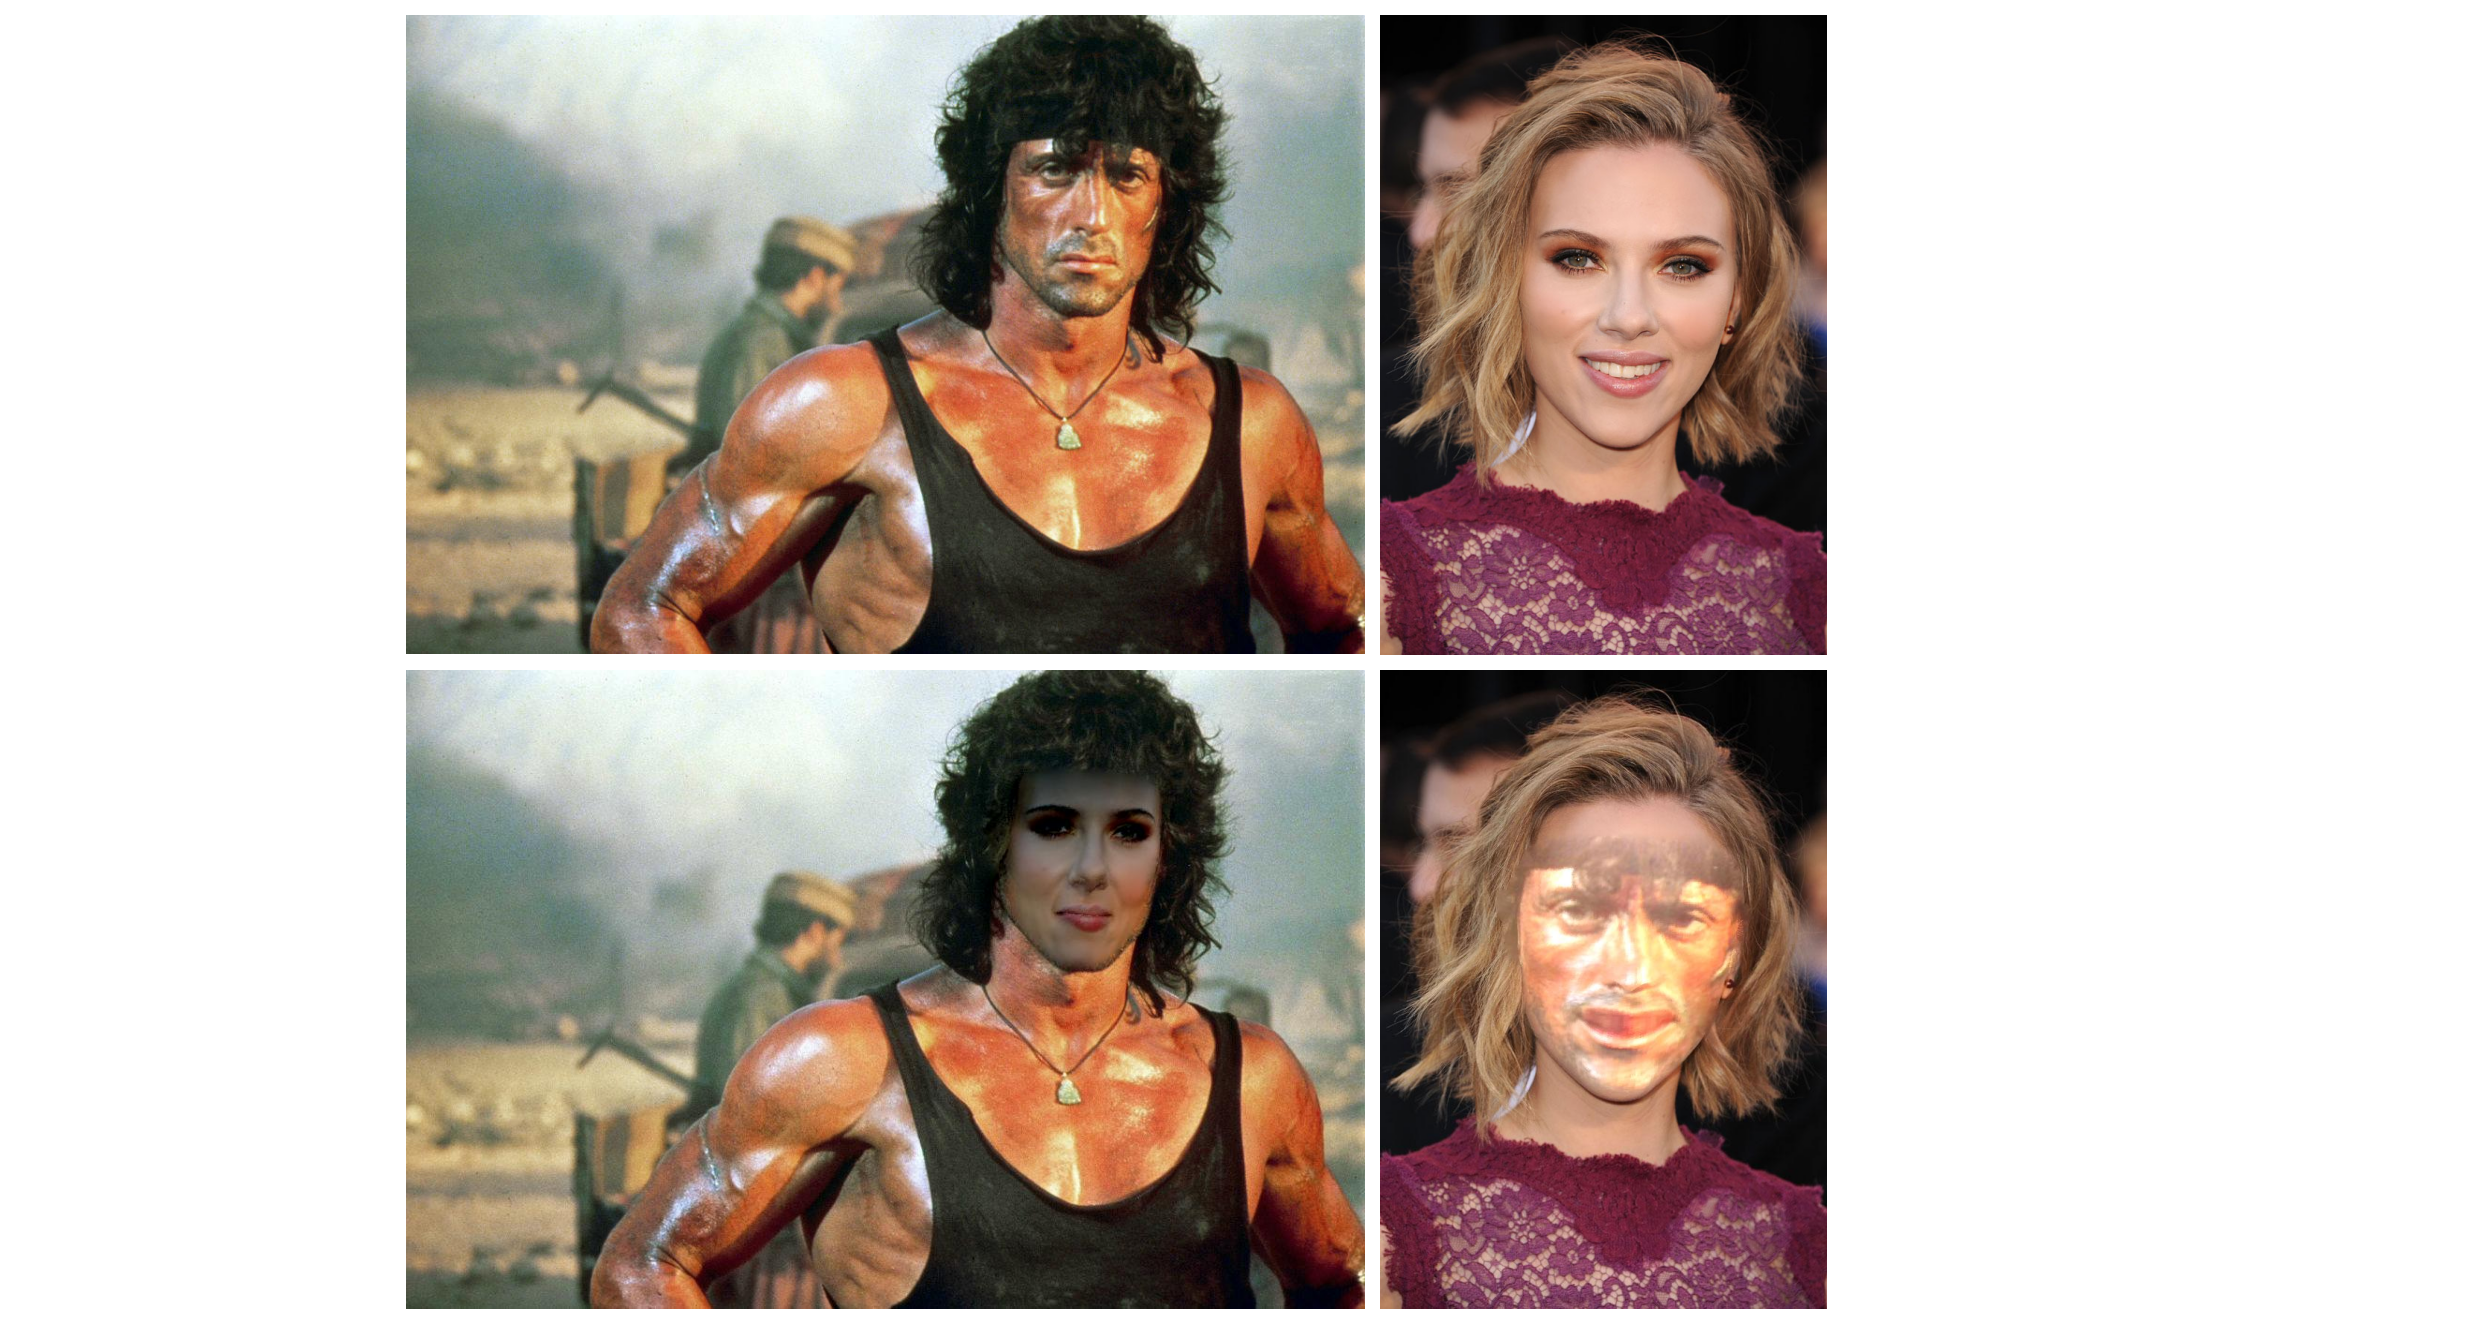
\includegraphics[width=0.5\textwidth]{Rambo_Johansson.png}
\centering
\caption{Images in the test set and their swaps}
\end{figure}

\begin{figure}[H]
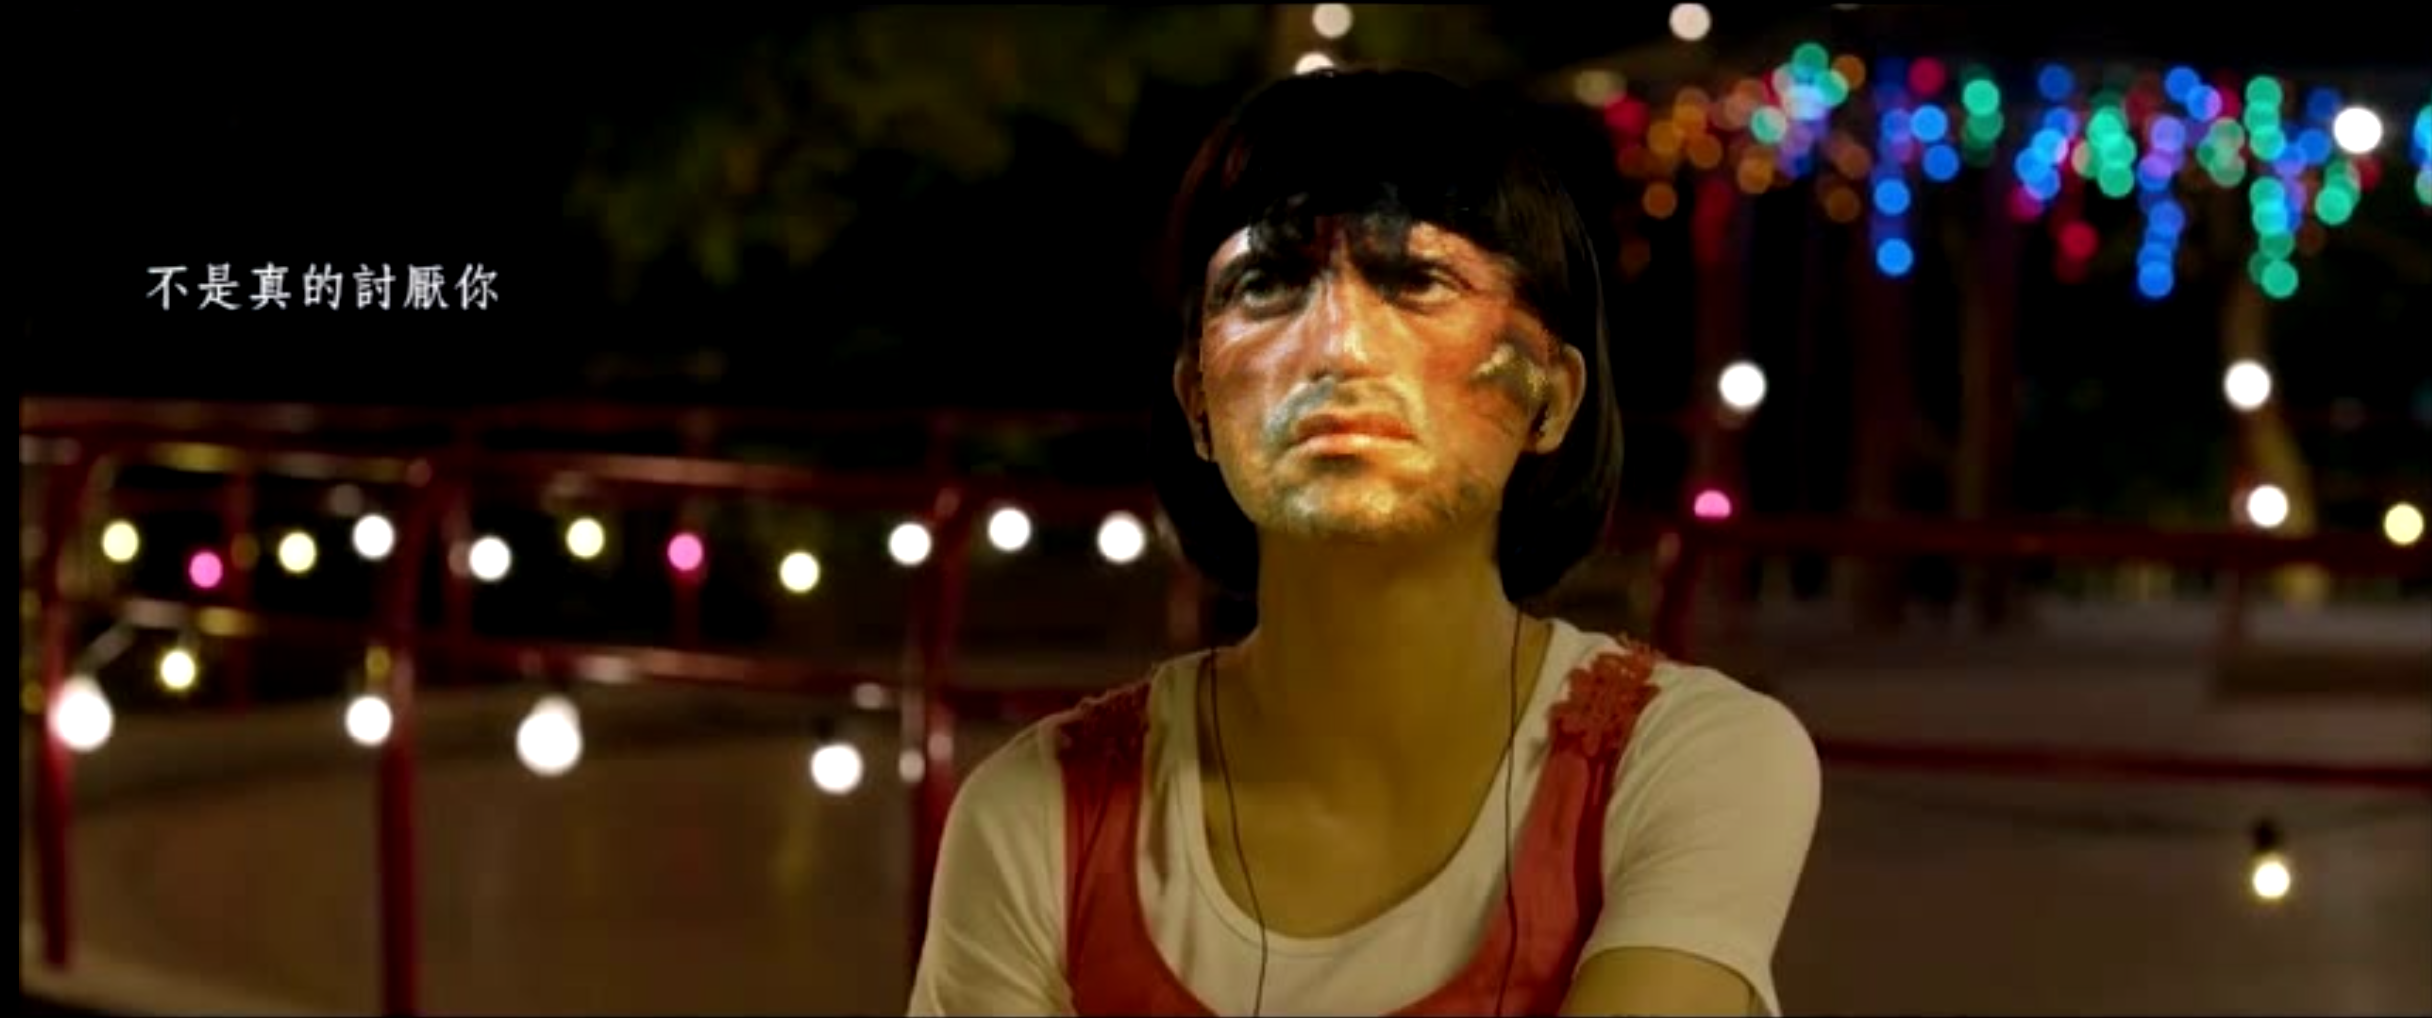
\includegraphics[width=0.5\textwidth]{korambo.png}
\centering
\caption{Faceswap in Test Video1}
\end{figure}


\begin{figure}[H]
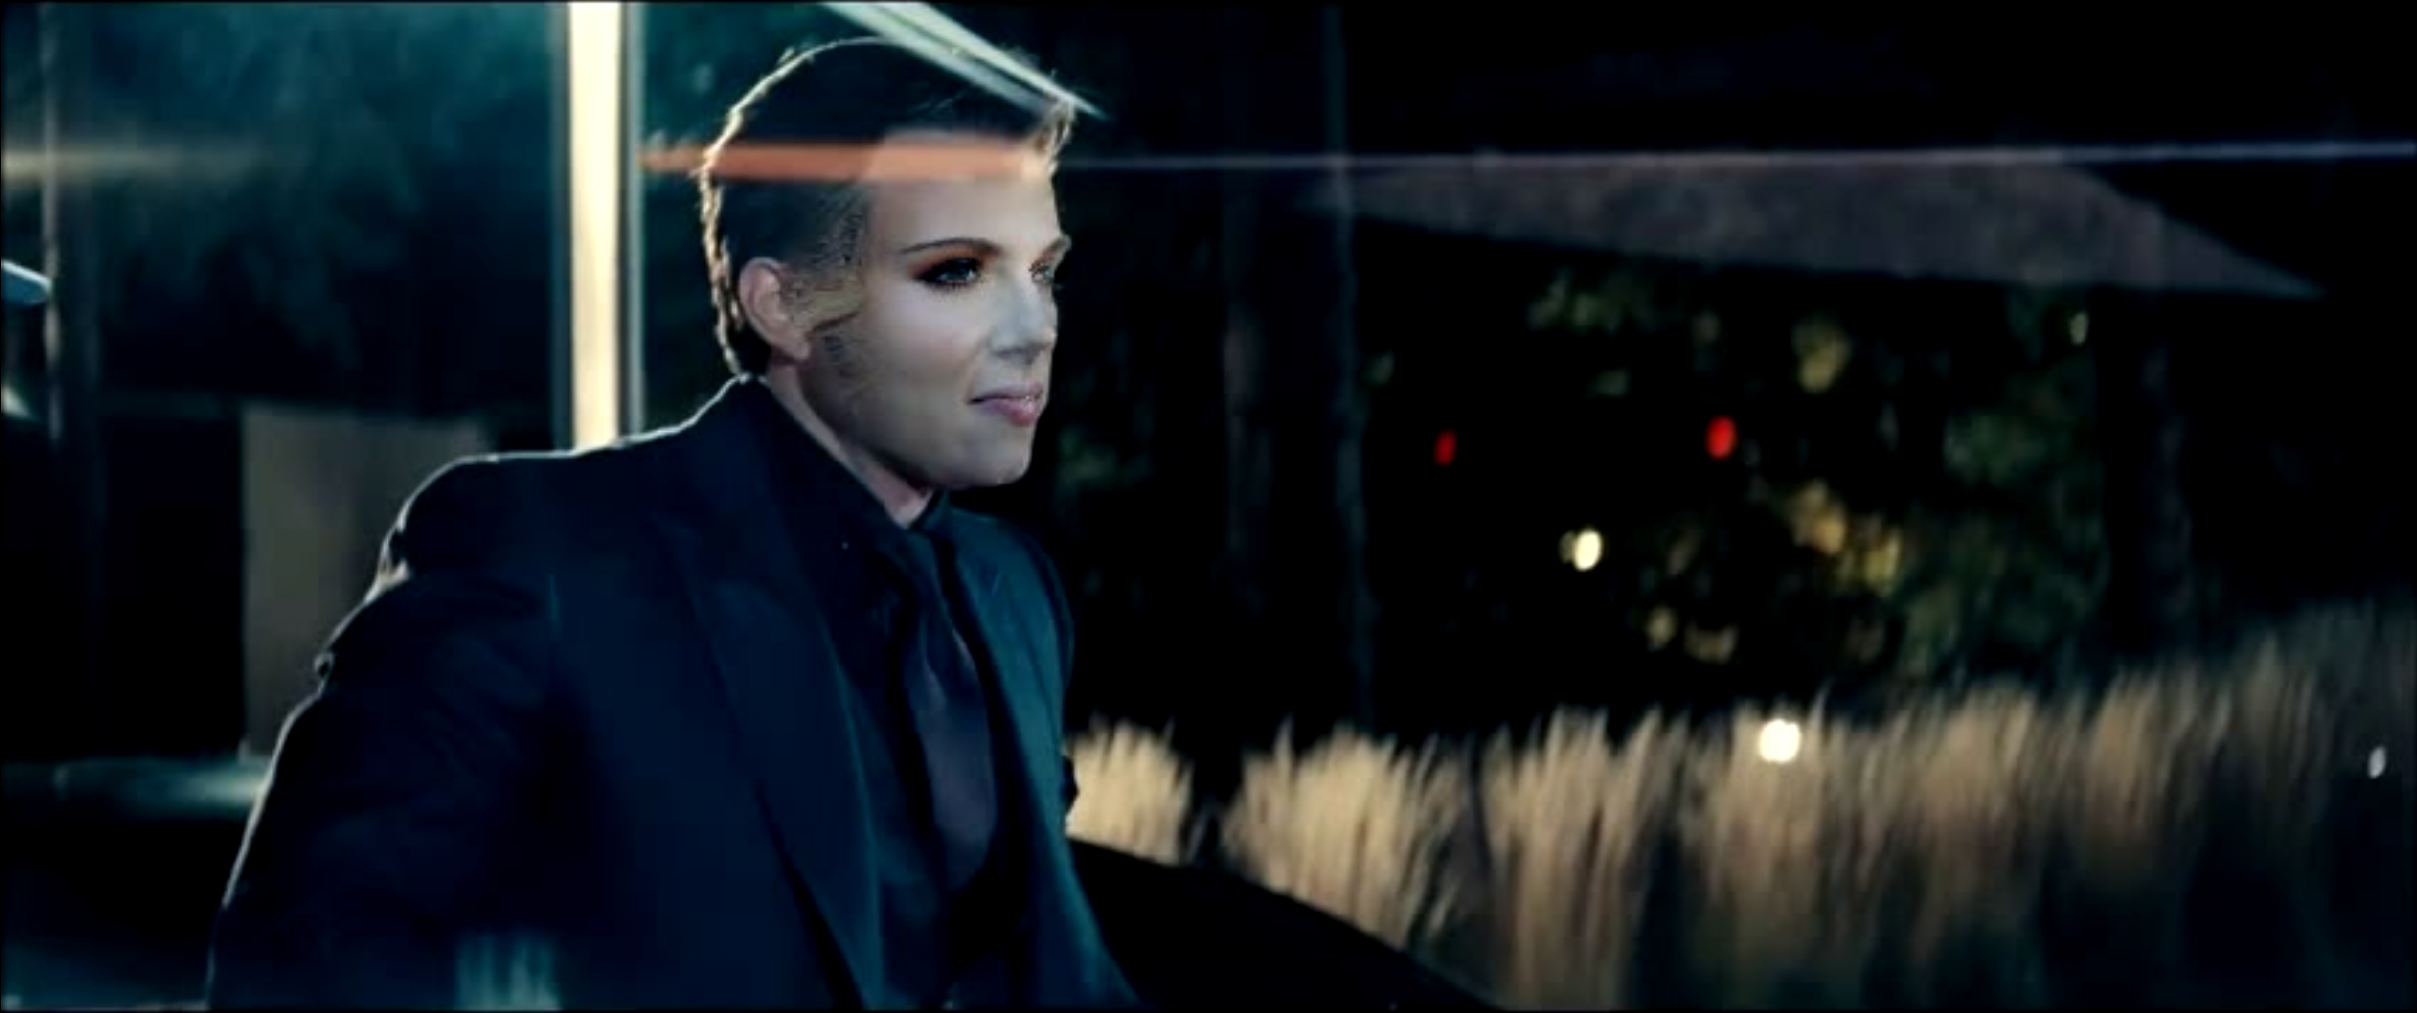
\includegraphics[width=0.5\textwidth]{scarbat.png}
\centering
\caption{Faceswap in Test Video3}
\end{figure}

\begin{figure}[H]
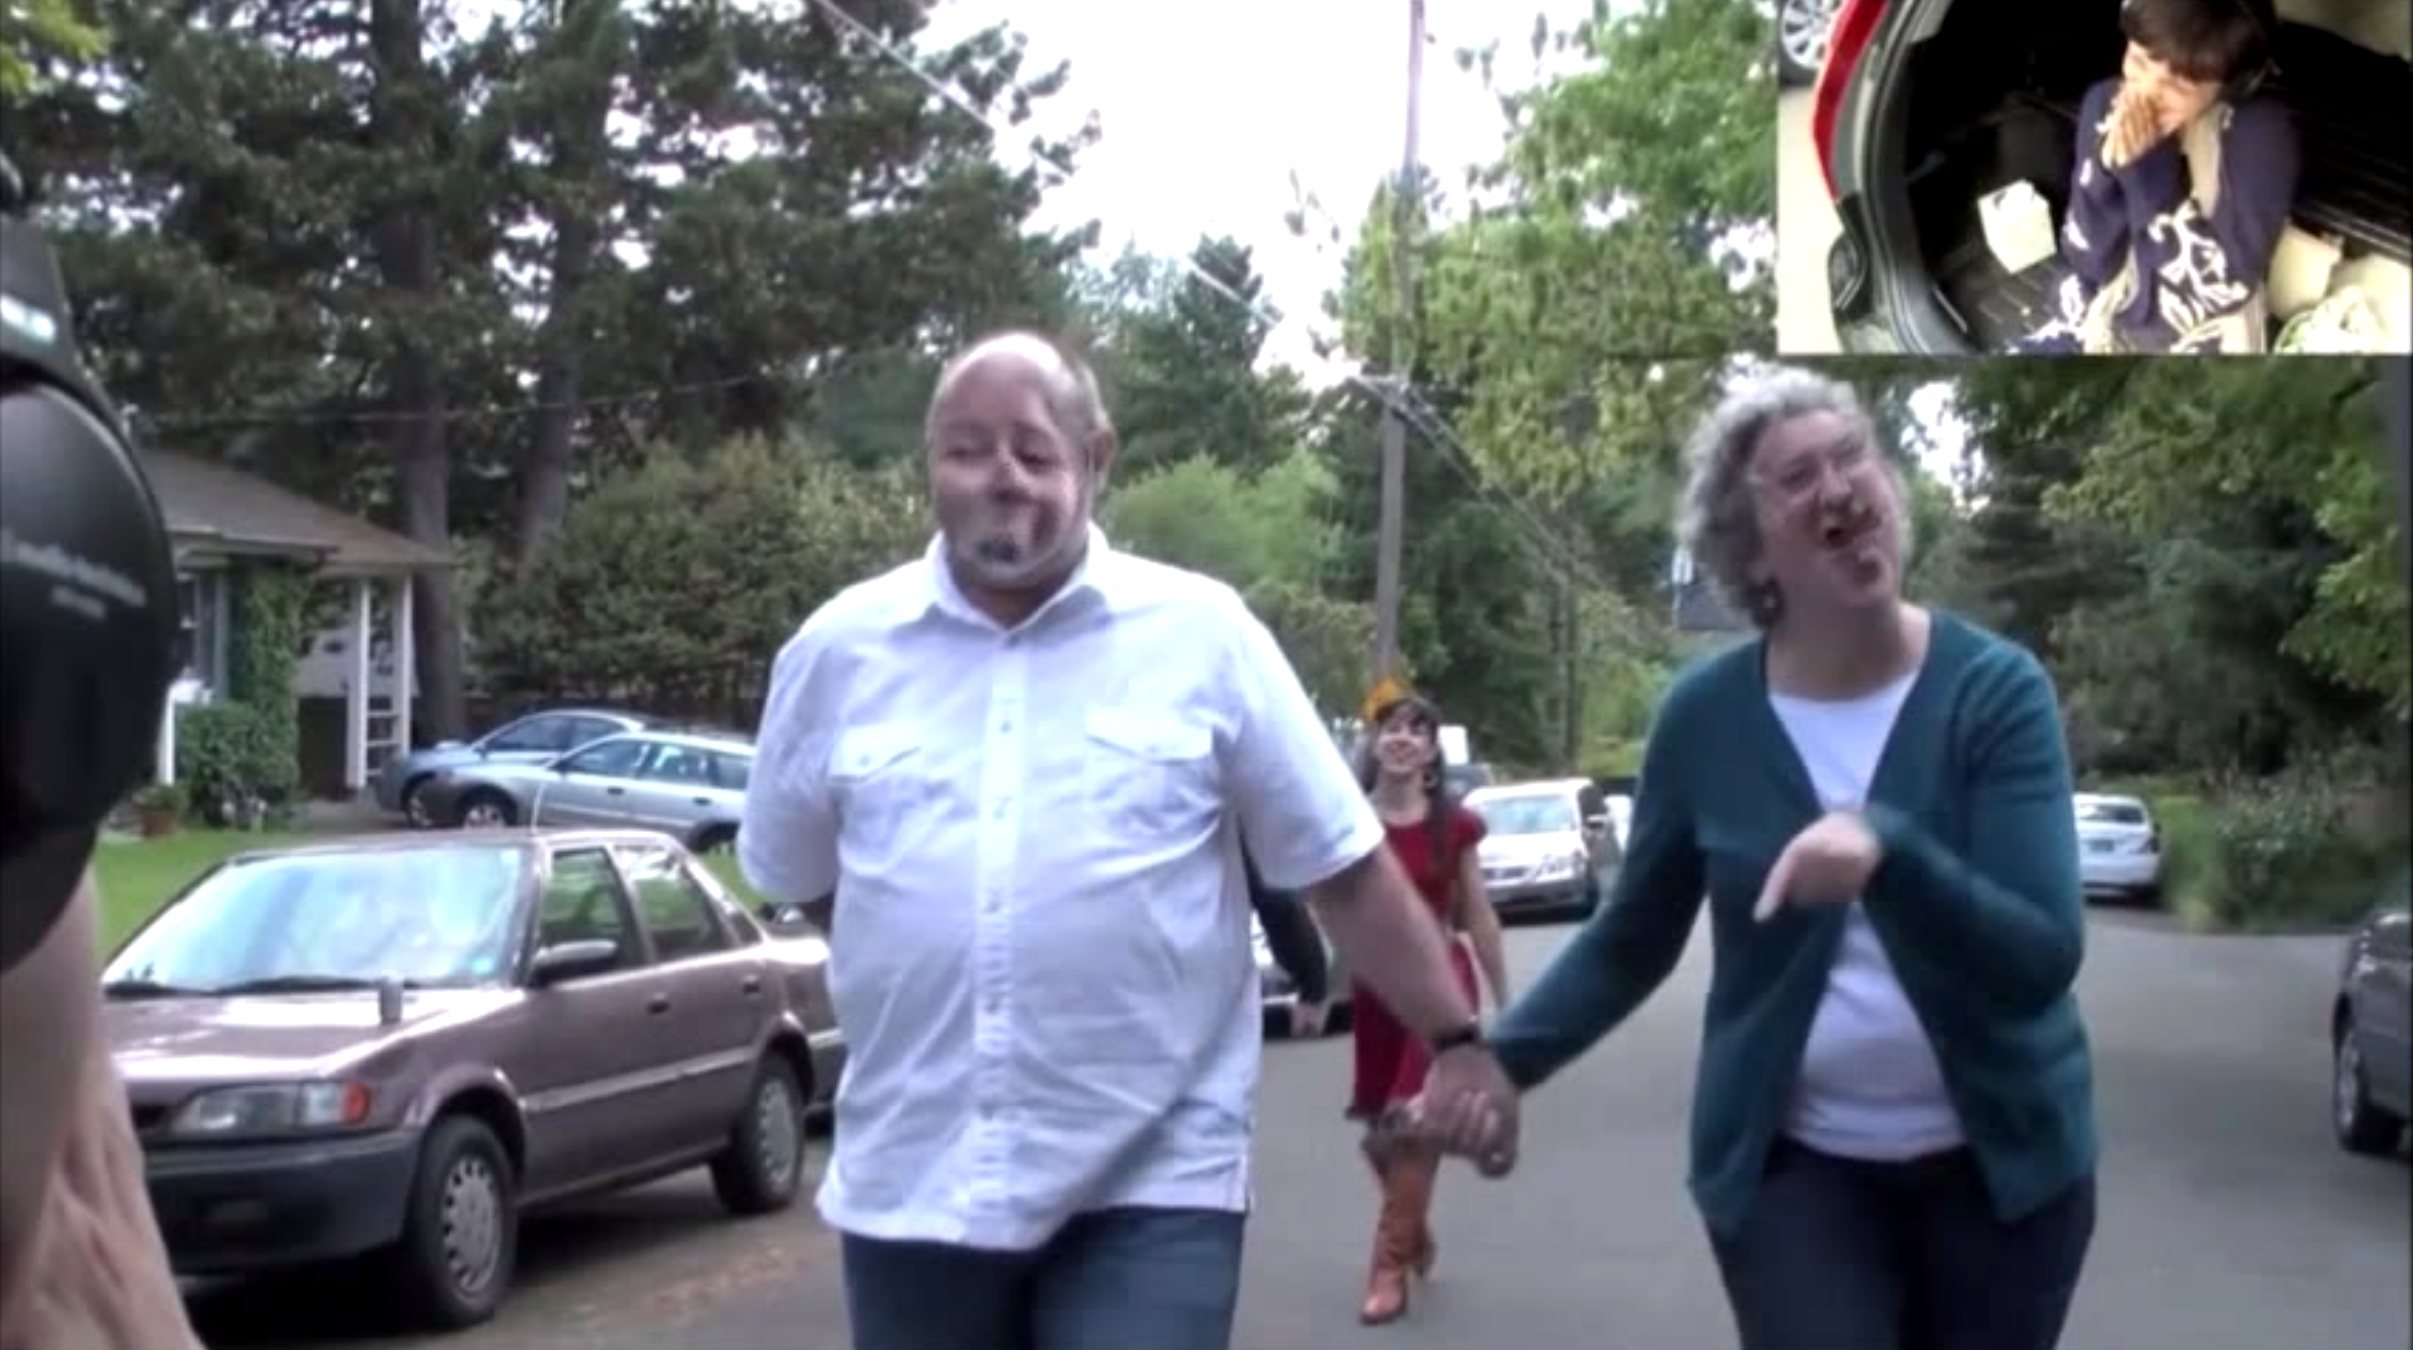
\includegraphics[width=0.5\textwidth]{couple.png}
\centering
\caption{Faceswap within Test Video2}
\end{figure}

It must be noted that the presence of facial hair and the hair on the refrence as well as the recepient's head plays a major role in the quality of the faceswap. Further we also noticed that the direction in which the recepient and reference faces are looking are also quite important, as this causes problems as seen above. Finally, varioation in skin tones also presents a major challenge.

In Test video 3, it was noticed that there were two extreme cases of lighting - too low or when cameras flash, too high, which hindered the detecion of images, for this we performed histigram equalization of the said frame and were able to improve the performance.

Finally, we applied our code on a video of our own recording. The result for this can be observed below.

\begin{figure}[H]
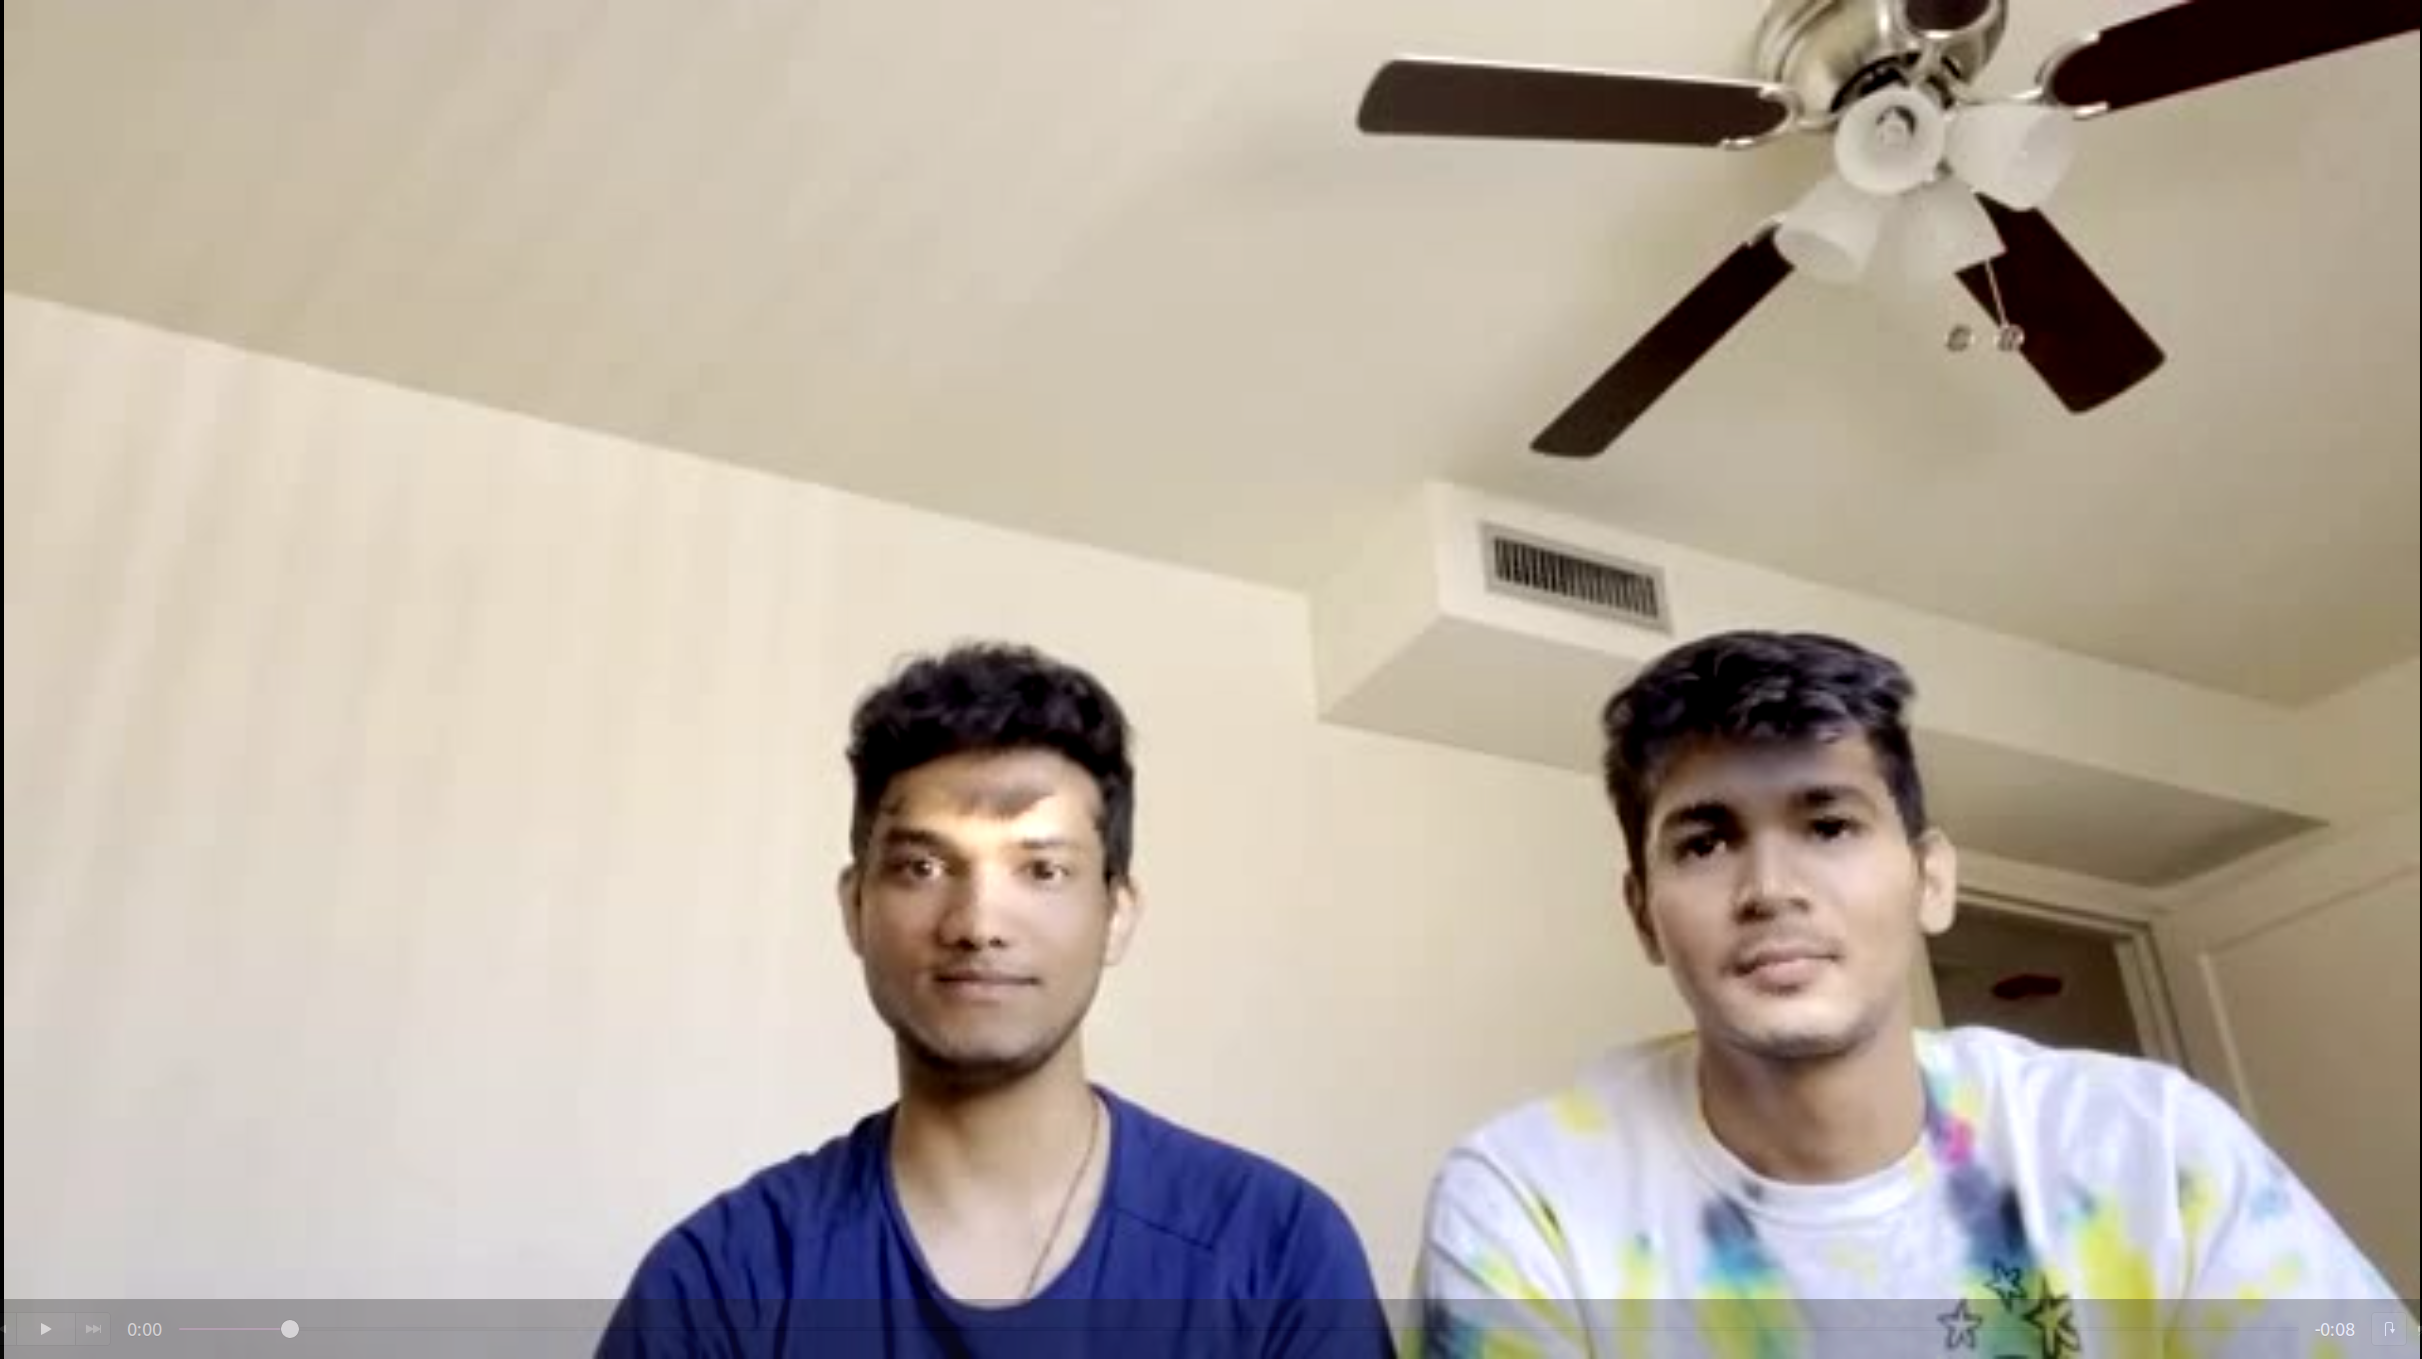
\includegraphics[width=0.5\textwidth]{palande.png}
\centering
\caption{Faceswap within Data Video2}
\end{figure}

\begin{thebibliography}{1}
\bibitem{1}{'Joint 3D Face Reconstruction and Dense Alignment with Position Map Regression Network'; Yao Feng, Fan Wu, Xiaohu Shao, Yanfeng Wang, Xi Zhou}
\bibitem{2}{https://github.com/YadiraF/PRNet}


\end{thebibliography}




\end{document}


